\documentclass[12pt,a4paper]{scrartcl}

\usepackage{graphicx}
\usepackage{amsmath}
\usepackage{amsfonts}
\usepackage{amssymb}
\usepackage{bm}
\usepackage{ulem}
\let\mathbf\bm


\usepackage[T1]{fontenc}
\usepackage[utf8]{inputenc}
\usepackage[magyar]{babel}
\usepackage{lmodern}

\usepackage{placeins}
\usepackage{subcaption}
\usepackage{epstopdf}
\usepackage{xcolor}
\usepackage[locale=FR, exponent-product = \cdot]{siunitx}
\usepackage[hidelinks,unicode]{hyperref}
\hypersetup{
    colorlinks,
    linkcolor={red!50!black},
    citecolor={blue!50!black},
    urlcolor={blue!80!black}
}

\usepackage{cleveref}


\newcommand{\mom}{\mathbf p}	%impulzus
\newcommand{\prob}{\mathtt p}	%valószínűség
\newcommand{\pres}{\mathsf p}	%nyomás


\begin{document}
\title{Hőtan és folytonos közegek mechanikája\\(emelt szint)}
\author{hotanef19va, házi feladatok\\Anyagfizikai Tanszék, Tüzes Dániel}
\maketitle
\tableofcontents

\iffalse %csak akkor használd, ha nincs további if belül
\section{Sűrűséges feladatok}
\subsection{Rúd sűrűsége}
Egy rúd sűrűsége a hely függvényében legyen $\varrho \left( x \right) = c/{x^2}$.
\begin{enumerate}
\item Milyen típusú sűrűségre gondolt az, aki egy ilyen példát kitűz?
\item Mi lehet $c$ dimenziója?
\item Mi a rúd tömege a
\begin{itemize}
\item $\left[ 1{\text{ m, }}2{\text{ m}} \right]$,
\item $\left( 1{\text{ m, }}2{\text{ m}} \right)$,
\item ${\left( {0{\text{ m, }}1{\text{ m}}} \right)}$ és
\item ${\left[ {0{\text{ m, }}1{\text{ m}}} \right]}$ között?
\end{itemize}
\item Létezhet-e ilyen sűrűségű lemez?
\end{enumerate}
\subsection{Levegő sűrűsége}
A levegő sűrűsége legyen a $h$ magasság függvényében $\varrho \left( h \right) = {\varrho _0} \cdot {e^{ - c \cdot h}}$.
\begin{enumerate}
\item Mi $c$ és $\varrho_0$ dimenziója?
\item Hanyad részére csökken adott térfogatú levegő tömege $L$-lel magasabban, ha a térfogat befoglaló gömbjének átmérője $ \ll \frac{1}{c}$?
\end{enumerate}

\subsection{Áramerősség}
Legyen az áramsűrűség-mező ${\mathbf{j}}\left( {\mathbf{r}} \right) = c \cdot {\mathbf{r}}/{r^3}$.
\begin{enumerate}
\item Mi $c$ dimenziója?
\item Mennyi töltés halad át az $1\text{ m}$ sugarú gömbön? És a $2\text{ m}$ sugarún?
\item Mennyi töltés halad át azon a négyzeten, aminek a négy sarkának a koordinátái: ${{\mathbf{r}}_A} = \left( {1,0,0} \right)$, ${{\mathbf{r}}_B} = \left( {1,1,0} \right)$, ${{\mathbf{r}}_C} = \left( {1,1,1} \right)$ és ${{\mathbf{r}}_D} = \left( {1,0,1} \right)$?
\end{enumerate}
\fi

\section{Merev testek}
\subsection{Négyféle tenzor}
\includegraphics[scale=0.8]{lusta/merev_test1pelda.png}

A c) és d) alfeladatokhoz számold ki az egyik $M$ tömegű testbe helyezett origóra a tehetetlenségi nyomaték tenzort az a) és a b) esetekben párhuzamos tengelyekre!

\subsection{Integrális rúd}
\includegraphics[scale=0.8]{lusta/merev_test2pelda.png} 

A rúd elég vékony, a hossztengelye mentén egy szakasszal modellezhető ebben a feladatban.

\section{Egyszerű transzformációk I}
\subsection{Eltolás otthon}
Legyen a testünk $A$ és $B$ pontjainak koordinátáira ${{\mathbf{r}}_A} = \left( { - 10, - 1} \right)$ és ${{\mathbf{r}}_B} = \left( { 3, 3} \right)$, valamint $\Delta {\mathbf{r}} = {{\mathbf{r}}_B} - {{\mathbf{r}}_A}$! Legyen az elmozdulásmező ${\mathbf{u}}\left( {\mathbf{r}} \right) = \left( { - 2, - 2} \right)$. Mennyi a disztorzió és annak szimmetrikus illetve antiszimmetrikus része, a deformációs gradiens, a deformáció és a relatív térfogatváltozás? Számold ki $\Delta {\mathbf{r}}'$ értékét is!

\subsection{Nyújtás otthon}
\begin{enumerate}
\item Legyen a testünk $A$ és $B$ pontjainak koordinátáira ${{\mathbf{r}}_A} = \left( { - 3, - 0.5, 0} \right)$ és ${{\mathbf{r}}_B} = \left( { - 0.5, - 0.5, 0} \right)$, valamint $\Delta {\mathbf{r}} = {{\mathbf{r}}_B} - {{\mathbf{r}}_A}$! Végezzünk el a testünkön egy transzformációt, amelynek során minden régi ${\mathbf{r}} = \left( {x,y,z} \right)$ helyvektor az alábbi ${\mathbf{r}}' = \left( {x',y',z'} \right)$ helyvektorba megy át: 
\[\begin{aligned}
  x' &  = 2 \cdot x \\ 
  y' &  = \lambda \cdot y \\ 
  z' &  = \lambda  \cdot z. \\ 
\end{aligned} \]

Mennyi a disztorzió és annak szimmetrikus illetve antiszimmetrikus része, a deformációs gradiens, a deformáció és a relatív térfogatváltozás? Add meg $\Delta {\mathbf{r}}'$ értékét is!

Mennyi legyen $\lambda$, hogy a relatív térfogatváltozás 0 legyen? Mennyi ekkor a disztorzió és annak szimmetrikus illetve antiszimmetrikus része, a deformációs gradiens, a deformáció? Add meg $\Delta {\mathbf{r}}'$ értékét is és készíts rajzot!

\item Legyen a testünk $A$ és $B$ pontjainak koordinátáira ${{\mathbf{r}}_A} = \left( { - 3, - 0.5, 0} \right)$ és ${{\mathbf{r}}_B} = \left( { - 0.5, - 0.5, 0} \right)$, valamint $\Delta {\mathbf{r}} = {{\mathbf{r}}_B} - {{\mathbf{r}}_A}$! Végezzünk el a testünkön egy transzformációt, amelynek során minden régi ${\mathbf{r}} = \left( {x,y,z} \right)$ helyvektor az alábbi ${\mathbf{r}}' = \left( {x',y',z'} \right)$ helyvektorba megy át: 
\[\begin{aligned}
  x' &  = 2 \cdot x \\ 
  y' &  = 3 \cdot y \\ 
  z' &  = 1 \cdot z. \\ 
\end{aligned} \]

Írd fel az elmozdulásmezőt vektoros alakban! Mire változik a $\Delta {\mathbf{r}}$ vektor? Mennyi a disztorzió, a deformációs gradiens és a relatív térfogatváltozás?

Tegyük át és rögzítsük az origót az anyagon az $A$ ponton és írjuk le innen is a nyújtást! Legyenek a vektoraink a csillagosak, ${{\mathbf{r}}_A}^*$ és ${{\mathbf{r}}_B}^*$. Hogyan változnak transzformációra általánosan a vektorok? Azaz add meg az ${\mathbf{r}}{{^*}'}\left( {{{\mathbf{r}}^ * }} \right)$ függvényt! Mi az elmozdulástér, a disztorzió, a $\Delta {{\mathbf{r}}^ * }'$, a deformációs gradiens, a deformáció és a relatív térfogatváltozás? Készíts rajzot is!
\end{enumerate}


\section{Egyszerű transzformációk II}
\subsection{Konkrét számok}
Írd fel az alábbi esetekre az elmozdulásmezőt, a disztorziót, a deformációs gradienst és a deformációt! Hogyan néznek ki ezek (első rendű közelítésben), ha a disztorziót egy $\varepsilon$ kicsi szám paraméterezi\footnote{Pontosabban szólva a disztorzió a paraméter 0 értéke mellett a konstans 0, a paraméter 1 értéke mellett az eredeti disztorzió, a paraméter $1/n$ értéke mellett $n$-szer kell ismételni az operációt a módosított disztrozióval ($n \in \mathbb{N}$), hogy az eredeti transzformációt megkapjuk, illetve $n_1/n_2$ esetben pedig a szükséges $n_2$ alkalomból $n_1$-szer már megismételtük.}?

\begin{figure}[htb] 
\centering
\begin{subfigure}[b]{0.45\textwidth}
\centering
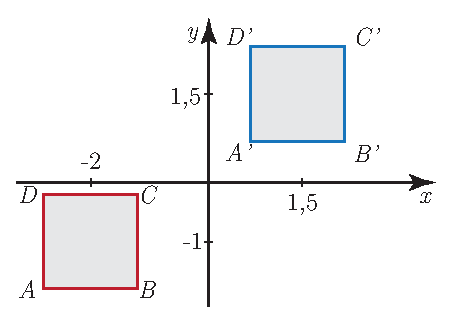
\includegraphics[scale=1]{figs/eltolas_feladat.eps}
\caption{Eltolás.}
\label{fig:eltolas_feladat}
\end{subfigure} \hfill
\begin{subfigure}[b]{0.45\textwidth}
\centering
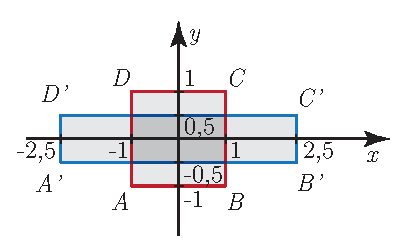
\includegraphics[scale=1]{figs/nyujtas_feladat.eps}
\caption{Nyújtás.}
\label{fig:nyujtas_feladat}
\end{subfigure}
\begin{subfigure}[b]{0.45\textwidth}
\centering
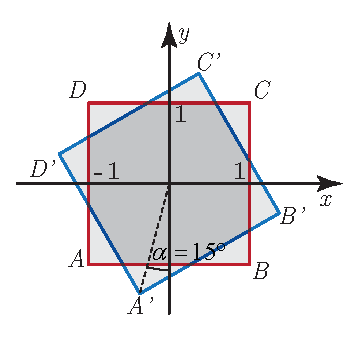
\includegraphics[scale=1]{figs/forgatas_feladat.eps}
\caption{Forgatás.}
\label{fig:forgatas_feladat}
\end{subfigure}
\label{fig:konret_szamos_feladat}
\caption{Konkrét számos feladat.}
\end{figure}
\FloatBarrier

\subsection{Egyenes képe egyenes}
Mutassuk meg, hogy eltolás, nyújtás és forgatás során szakasz képe szakasz! Ehhez felhasználhatjuk, hogy az $A$ és $B$ pontok közötti $AB$ szakaszt a két pontba mutató ${{\mathbf{r}}_A}$ és ${{\mathbf{r}}_B}$ vektorokkal úgy írhatjuk fel, hogy 
\[AB = \left\{ {\left. {{\lambda _A}{{\mathbf{r}}_A} + {\lambda _B}{{\mathbf{r}}_B}} \right|{\lambda _A} + {\lambda _B} = 1} \right\}.\]

\subsection{Nyírós-számolós}
\begin{enumerate}
\item \Aref{fig:nyiras_feladat}.\ ábrán melyik fajta nyírás van ábrázolva? Mi az elmozdulásmező, a deformációs gradiens, a disztorzió és a deformáció?
\item Legyen egy négyzet oldalai párhuzamosak a vonatkoztatási rendszerrel, és legyen a szimmetriatengelyeiben az origó! Egyszerű nyírás esetén kifejezhetőek-e a disztorzió egyes komponensei a transzformációt bemutató ábráról leolvasható szögek függvényében? Hogyan változik a kifejezés infinitezimális transzformáció esetén?

Extra gondolkodó házi feladaton kívül: tiszta nyírás esetén kifejezhető-e az ábráról leolvasható szögek függvényeivel, hogy mely tengely menti mekkora nyújtást ír le a transzformáció, ha az ábrán Euklideszi szerkesztést is engedélyezünk? Hogyan módosul a kifejezés infinitezimális transzformációra?
\item Infinitezimális tiszta nyírásnál elsőrendig nézve hogyan néz ki az elmozdulásmező, a deformációs gradiens, a disztorzió és a deformáció abban a vonatkoztatási rendszerben, amelyben ${\mathbf{F}}$ diagonális? Hogyan néznek ki ugyanezek a mennyiségek $45^\circ$-os szöget bezáró koordinátarendszerben?
\end{enumerate}


\begin{figure}[htb] 
\centering    
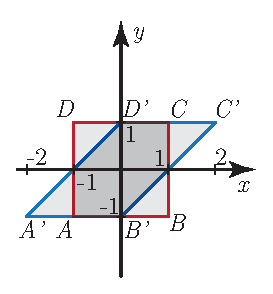
\includegraphics[scale=1]{figs/nyiras_feladat.eps}
\caption{Nyírós feladat.}
\label{fig:nyiras_feladat}
\end{figure}
\FloatBarrier

\section{Összetett vagy nemhomogén transzformációk}
\subsection{Homokóra nyújtós}
Mi az elmozdulásmező, a deformációs gradiens, a disztorzió és a deformáció \aref{fig:homokora_nyujtas_feladat}.\ ábrán?

\begin{figure}[htb] 
\centering    
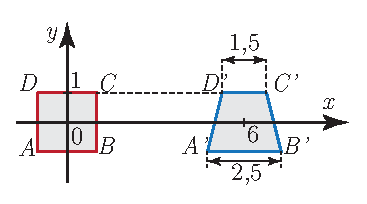
\includegraphics[scale=1]{figs/homokora_nyujtas_feladat.eps}
\caption{Homokóra nyújtós feladat.}
\label{fig:homokora_nyujtas_feladat}
\end{figure}
\FloatBarrier

\subsection{Visszafejtés}
Milyen transzformációkat takarnak az egyes deformációs gradiensek? Mekkora forgatást és milyen tengely irányú mekkora nyújtást vagy nyírást tartalmaznak? Rajzold le, mivé transzformálódik az egységnégyzetet, és jelöld be rajta a nyújtás tengelyeit és a forgatás szögét, ha van!

\[{{\mathbf{F}}_1} = \left( {\begin{array}{*{20}{c}}
  {\sqrt 2 }&-{\sqrt 2 } \\ 
  {\sqrt {0{,}125} }&{ \sqrt {0{,}125} } 
\end{array}} \right)\quad {{\mathbf{F}}_2} = \left( {\begin{array}{*{20}{c}}
  {1{,}2}&0 \\ 
  0&{1{,}5} 
\end{array}} \right)\quad {{\mathbf{F}}_3} = \left( {\begin{array}{*{20}{c}}
  2&{0{,}2} \\ 
  {0{,}2}&{0{,}5} 
\end{array}} \right)\]


\section{Folytonos közegek egyensúlya}

\subsection{Oszlopban állandó feszültség}
Egy állandó $\varrho$ sűrűségű, hossztengelyére forgásszimmetrikus test (olyan oszlop, amelynek a hossztengelyére merőleges keresztmetszete minden magasságban kör) felső lapja a felfüggesztéshez van rögzítve, alsó síklapjára egy $G$ súlyú nehezék van rögzítve. Milyen alakú legyen az oszlop, hogy a feszültségtenzor hossztengellyel párhuzamos $\sigma_{zz}$ komponense állandó legyen azon belül?

\subsection{Csöves 1}
Mekkora a másodrendű nyomatéka egy tömör hengernek a hossztengelyére merőleges keresztmetszetében? Hogyan aránylik ez egy azonos nagyságú keresztmetszettel rendelkező üreges csőéhez képest, ugyanolyan irányú keresztmetszetben, ha a cső külső sugara kétszerese a tömör hengernek?

\subsection{Húzódzkodó}
2 db négyzetes profilú, \SI{3}{cm} oldalélű, valamilyen anyagvastagságú hasáb tart egy húzódzkodó keresztrudat a faltól \SI{50}{cm} távolságban. Mekkora a négyszögletes vas rudak anyagvastagsága, ha Gyurma Gyuri a maga \SI{80}{kg}-os testtömegével a keresztrúdra ráfüggeszkedvén annak lehajlása \SI{5}{mm}? A vas Young-modulusza \SI{200}{GPa}.

\section{Hidrosztatika és felületi feszültség}
\subsection{Parafa-rugó}
Egy vízzel telt edénybe $d$ átmérőjű, $\varrho$ sűrűségű ($\varrho<\varrho_{\text{víz}}$) parafagolyót helyezünk, majd az edény aljához kötjük egy $D$ rugóállandójú rugóval. Mekkora a rugó megnyúlása, ha a golyó teljes egészében a folyadékban van?


\subsection{Lapát}
Egy lapát sűrűségét szeretnénk meghatározni azáltal, hogy tudjuk, hogy egyik végénél fogva, a vízbe ferdén belelógatva épp a lapát hosszának felénél van a vízszint. Ehhez azt a modellt használjuk, hogy a lapát és a víz sűrűsége állandó, alakja \sout{kecses} vékony rúd, amelynek a vastagsága elhanyagolható, továbbá a lapátot tartó kezünk gömbcsuklóként, egyetlen pontban tartja a lapátot.

\subsection{Türelem}
Két, közel azonos méretű szappanbuborék gömböt fújunk fel egy Y alakú csővel, majd a buborékok közötti levegő áramlását a felfújást követően is biztosítjuk. Tegyük fel, hogy az egyik buborékból a másikba történő anyagáramlás sebessége elég lassú és arányos a buborékokban mérhető nyomás különbségével, ${\dot m_1} = \beta  \cdot \left( {{p_2} - {p_1}} \right)$, a $T$ hőmérséklet állandó, a cső térfogata elhanyagolható a buborékokéhoz képest, valamint tekintsük a levegőt ideális gáznak! 

\begin{enumerate}
\item Írjuk fel a szappanbuborék átmérőjének időbeli változására a differenciál- és algebrai egyenletet úgy, hogy csak a szappanbuborékok sugara maradjon meg, mint időfüggő mennyiség!
\item Legyen az egyenlő sugarú esetben a buborékok (instabil) egyensúlyi sugara $R$! Mutassuk meg, hogy amennyiben $R_1 = R + \varepsilon_1$ és $R_2 = R - \varepsilon_2$, ahol $\varepsilon_1$ és $\varepsilon_2$ elég kicsi, akkor $\varepsilon_1/\varepsilon_2=1$!
\item Írjuk fel a differenciálegyenletet az instabil egyensúlyi helyzet körül, $\varepsilon$-ban elsőrendig közelítve! Oldjuk meg a differenciálegyenletet! Ezzel a közelítéssel számolva mennyivel több időt kell várni, amíg $\varepsilon/R$ megnő $1$-ről $2\%$-ra, ahhoz képest, mintha $2$-ről $3\%$-ra növekedne?
\item Extra gondolkodó 1 (házi feladatokon kívül): Mekkora lesz a nyomás a felfújt szappanbuborékban és mekkora lesz a sugara, ha az instabil egyensúlyi helyzethez tartozó sugár $R$, és eltekintünk a görbületi nyomás járulékától a külső nyomáshoz képest? Mennyivel változik meg ehhez képest a felfújt szappanbuborékhoz tartozó sugár első rendben, ha nem hanyagoljuk el a görbületi nyomást a külső nyomáshoz képest?
\item Extra gondolkodó 2 (házi feladatokon kívül): hogyan csökken 0-ra a kisebbik gömb sugara? Vizsgáljuk meg azt a határesetet, amikor az egyik gömb már majdnem teljesen fel van fújva, a másik pedig már nagyon kicsi!
\end{enumerate}

\section{Folyadékok II}
\subsection{BernoUlli}
Egy szögletes, alul vízszintes, oldalt függőleges szárú, U alakú, két végén nyitott csőben folyadék van (lásd \aref{fig:ucsoves}.\ ábrát). A cső vastagsága elhanyagolható a hosszához képest. A csövet az U egyik szára tengelyében állandó $\omega$ szögsebességgel forgatjuk. A forgástengelyhez közelebbik vízszint helyzetét jelöli $A$, a forgástengelytől távolabbikat $B$. Hogyan viszonyul a vízszint különbsége az $A$ és $B$ pontok között az $\omega$ szögsebesség függvényében?

\begin{figure}[htb] 
\centering    
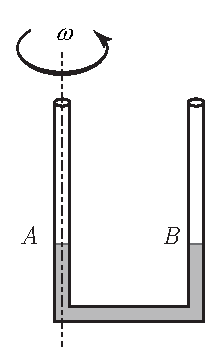
\includegraphics[scale=1]{figs/bernoUlli.eps}
\caption{Egy U alakú csőben folyadék van egyensúlyban, majd megforgatjuk a csövet az U egyik szára tengelyében.}
\label{fig:ucsoves}
\end{figure}
\FloatBarrier

\subsection{Csöves 2}
Egy U alakú, $d$ átmérőjű, kör keresztmetszetű nyitott csőben folyadék van, $L$ hosszban, $d \ll L$. Az egyik csövön egy pillanatra levegőt befújva egy kicsit lecsökkentjük a folyadékszint magasságát $x_0$-val, majd figyeljük a vízszint mozgását. Milyen mozgást fog végezni? Tételezzük fel, hogy a cső adott keresztmetszete mentén lévő folyadékrészre a sebességével arányos súrlódási erő lép fel.
\begin{figure}[htb] 
\centering    
\includegraphics[scale=1]{figs/ucsoves2.pdf}
\caption{Egy U alakú csőben már megint folyadék van.}
\label{fig:ucsoves2}
\end{figure}
\FloatBarrier

\section{Gázok állapotegyenlete}
\subsection{Ideális példa}
A $V$ térfogatú tartályban $T$ hőmérsékleten összekeverünk $m_1$, $m_2$, \ldots tömegű és rendre $M_1$, $M_2$, \ldots moláris tömegű ideális gázokat. Mutassuk meg, hogy a rendszer állapotegyenlete
\[\pres V = \frac{m}{M}RT\]
alakú, ahol $m$ a teljes tömeg, $M$ pedig egy effektív moláris tömeg! Fejezzük ki $M$ értékét! A levegőt ideális gázok ilyesfajta keverékének tekintve mennyi $M_{\text{levegő}}$ értéke?

\subsection{Csak a fele}
\SI{4}{mol}
 anyagmennyiségű van der Waals gázt tárolunk egy \SI{5}{literes}
  tartályban \SI{1}{MPa} nyomáson. A gáz anyagi paraméterei 
  $a=\SI{4e7}{N.cm^4/mol^2}$, 
  $b=\SI{40}{cm^3/mol}$. Mekkora lesz a gáz nyomása, ha a tömegének a felét lassan kiengedjük a tartályból, miközben a hőmérsékletét állandó értéken tartjuk? Mi lett volna az eredmény ideális gáz esetén?
  
\subsection{Kritikus példa}
Számoljuk ki a van der Waals-gáz kritikus pontját meghatározó nyomás, térfogat- és hőmérsékletértékeket az állapotegyenletéből! Írjuk fel az állapotegyenletet úgy, hogy az $a$, $b$, $m$, $n$ és $M$ paraméterek helyett az állapotjelzők kritikus ponthoz tartozó értékeit, azaz $\pres_\text c$, $T_\text c$ és $V_\text c$ használjuk!

\subsection{Extra gáz}
Hogyan olvashatóak le az $a$ és $n \cdot b$ paraméterek a van der Waals gázok nyomás-térfogat diagramjáról, ha sok, különféle hőmérsékletre meg vannak adva az izotermák?

\paragraph{Extra feladat a házi feladatokon túl}
Hogyan változnak az izotermák az $a$ és $b$ paraméterek függvényében? Írjunk szkriptet, ami előállítja a van der Waals gáz izotermáit, és a különféle paraméterek mellett készített diagramokat animált gifbe összeillesztve készítsünk animációt, midőn $a$ felmegy 0-ról $p \cdot V^2/n^2$-ig, majd $b$ 0-ról $V/n$-ig, majd $a$ lemegy 0-ba, végül $b$ is lemegy $0$-ba! (A tartományok csak tippek, lehet, hogy más értékek mellett látványosabb az animáció.)

\section{Termodinamika I}
\subsection{Kvázisztatikus, nyomás}
Ideális gáz $\pres_1$ nyomású, $V_1$ térfogatú állapotából, szabad adiabatikus tágulás során a $\pres_2$ nyomású és $V_2 > V_1$  térfogatú állapotba jut. Ezután állandó nyomáson, kvázisztatikusan $V_1$  térfogatúra nyomjuk össze, majd ugyancsak kvázisztatikusan addig melegítjük, amíg a nyomása ismét $\pres_1$ nem lesz. Nyílt- vagy körfolyamatról van-e szó? Rajzoljunk ábrasorozatot az egyes állapotokhoz tartozó mennyiségeket is jelölve! Határozzuk meg a folyamat során leadott hőmennyiséget! Mely egyenleteken és hogyan kell módosítani, ha nem ideális gázunk van?
\subsection{Durrants be!}
A $V$ térfogatú hőszigetelt szobácska nem hermetikusan zárt, a külső nyomás $\pres$. Mennyi hő szükséges, hogy a szobában lévő levegő hőmérsékletét $T_1$-ről $T_2$-re emeljük? Tekintsük a levegőt ideális gáznak!
\subsection{Minden út \textit{B}-be vezet} % elmfiz 2: 13.10; KöMaL P. 4160.
\Atold\ref{fig:figizoterma_adiabata_AB}+as{} ábra egy ideális gáz állapotváltozásait mutatja. Mekkora a belős energia különbsége az $A$ és $B$ pontok között? Határozzuk meg a munkavégzést, ill.\ a felvett hőt az $A1B$, az $A2B$ és a $A3B$ kvázisztatikus folyamatokra! Adott a $C_v$ hőkapacitás és az $n$ anyagmennyiség.

\begin{figure}[htb] 
\centering   
\begin{subfigure}[b]{0.45\textwidth}
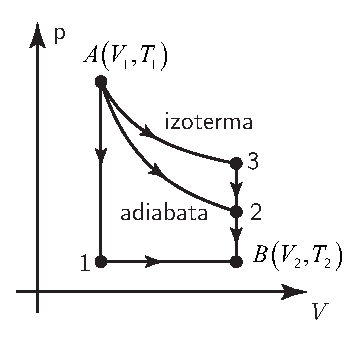
\includegraphics[scale=1]{figs/izoterma_adiabata_AB.eps}
\subcaption{Ideális gáz állapotváltoztatásai, amely során $A$-ból $B$-be jutunk el izobár, izoterm, izochor vagy adiabatikus módokon.}
\label{fig:figizoterma_adiabata_AB}
\end{subfigure} \hspace{2em}
\begin{subfigure}[b]{0.45\textwidth}
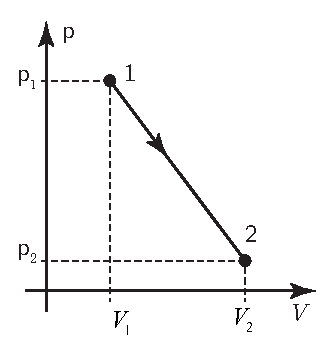
\includegraphics[scale=1]{figs/egy_ketto.eps}
\subcaption{Ideális gáz állapotváltozása, ami a $\pres - V$ síkon egyenes. Nem tartalmaz nevezetes részfolyamatot.\\}
\label{fig:egy_ketto}
\end{subfigure}
\end{figure}
\FloatBarrier

\subsection{Hosszú lesz}
Egy mólnyi ideális gázt \aref{fig:egy_ketto}.\ ábrán látható úton viszünk át kvázisztatikusan az 1-es állapotból a 2-es állapotba.
\begin{enumerate}
\item A folyamat mely részén lesz hőfelvétel és mely részén lesz hőleadás?
\item Határozzuk meg a gáz mólhőjét a folyamat során, ha ismert az állandó térfogat mellett mért mólhő! Lehet-e a folyamat során 0 a mólhő? Lehet-e végtelen?
\end{enumerate}

\section{Termodinamika II}
Tekintettel a május 7-ei oktatási szünetre, ezeket a házikat csak május 14-ig kell beadni, azonban már \textbf{délelőtt 10 órára be kell érkeznie}, hogy az utolsó órán lehessen a megoldásokról kérdezni.
\subsection{Kikondenzálódott} % elmfiz 2; 13.14
Kondenzált anyagok egy modelljében a nyomásra és a belső energiára a következő összefüggést adják meg valamilyen $V<V_0$ térfogatra $\alpha$, $\chi$, $V_0$ és $C_V$ anyagi paraméterek mellett:
\[\pres = \frac{1}{\chi }\left( {1 + \alpha T - \frac{V}{{{V_0}}}} \right)\qquad U = {C_V}T + \frac{{{V_0}}}{{2\chi }}{\left( {1 - \frac{V}{{{V_0}}}} \right)^2}.\]
\begin{enumerate}
\item Mi $\alpha$ szemléletes jelentése? Vizsgáljuk meg $d\pres$ mennyiséget állandó nyomás mellett!
\item Mik az izotermák egyenletei? Rajzold le őket néhány különböző $T$-re!
\item Mennyi hőt vesz fel a rendszer, ha állandó $\pres$ nyomáson $V_1$-ről $V_2$ térfogatúra tágul? Adjuk meg $Q$-t, mint $V_2 - V_1$ (és az anyagi paraméterek) függvénye! \footnotesize Tippért nézz a példa végére.\normalsize
\item Fejezzük ki $C_\pres$-t, az állandó nyomáson mérhető hőkapacitást az állandó térfogaton mérhető hőkapacitással és a hőmérséklettel!
\item Milyen anyagi állandók esetén lesz a $C_\pres - C_V$ különbség elhanyagolhatóan kicsi?
\item Határozzuk meg az adiabaták egyenletét! \footnotesize Tippért nézz a példa végére.\normalsize% elmfiz 2; 13.20
\item Rajzoljuk fel a Carnot-körfolyamat $\pres - V$ diagramját, adjuk meg a görbék egyenletét az anyagi paraméterek, valamint  $T_1$ és $T_3$, továbbá $V_1$ és $V_2$ függvényében, ahol $T_1>T_3$, a körfolyamat során mérhető legnagyobb és legkisebb hőmérséklet értékek, $V_1$ a $T_1$ hőmérséklet tartozó legkisebb térfogat, és $V_2$ pedig a legnagyobb! 
\item Mutassuk meg, hogy egy izotermán felvett hő kifejezhető csupán a hőmérséklettel és a térfogatváltozással! \footnotesize Tippért nézz a példa végére.\normalsize
\item Mutassuk meg, hogy a rendszeren végzett Carnot-körfolyamat hatásfoka a legnagyobb és legkisebb hőmérséklettől ugyanúgy függ, mint ideális gázra!% elmfiz 2; 13.25
\item Az előző pont szerint felírtuk a $Q_{1 \to 2}$ hőfelvételt, amit egy izotermán számoltunk ki, ezért $U$-k különbségéből először kiesett a hőmérsékletfüggés, de a nyomáson (állapotegyenlet) keresztül újra bejött a hőmérsékletfüggés. Az előző pont(ok) számolását felhasználva írjuk fel egy izotermán a $\delta Q$ elemi hőfelvételt, azaz ha a 2-es és 1-es állapot nagyon közeli!

Írjuk fel most úgy is, hogy nem tartjuk állandó értéken a hőmérsékletet, hanem letérhetünk az izotermáról, és így nem 2-es állapotba, hanem egy $1^*$ állapotba kerülünk, ahol a hőmérséklet $dT$-vel, a nyomás $d\pres$-vel, a térfogat pedig $dV$-vel odébb van! Ez megadja $\delta Q$ értékét általános elemi állapotváltozás során. Alakítsuk úgy az eredményt, hogy  a hőmérsékletet és térfogatot használjuk csak!
\item Írjuk fel az elemi redukált hőt, azaz $\delta Q /T$-t, majd ennek integrálásával határozzuk meg az $S\left( {T,V} \right)$ entrópiafüggvényt, majd elimináljuk $T$-t a belső energia segítségével, hogy megkapjuk az entrópiát, mint az $S\left( {U,V} \right)$ függvényt! % elmfiz 2; 14.4
\end{enumerate}
\footnotesize Tippek, amiket csak akkor olvass, ha nem jutottál előre.
\begin{itemize}
\item Tipp3: írd fel a termodinamika I.\ főtételét, használd ki, hogy az elvégzett munkát ki tudod számolni, és hogy a belső energiaváltozást is meg tudod határozni. Az állapotegyenlet segítségével a $\pres$ és $V$-t egyszerre tudod eliminálni $Q$-ból, ha szeretnéd. Az itt keresett hőkapacitás pedig $\delta Q/dT$ állandó nyomás mellett.
\item Tipp6: A belső energia teljes differenciálját írd fel, és használd ki, hogy 0 a felvett hő! A kapott egyenletben a változók szeparálhatók, ha az állapotegyenlet segítségével eliminálod $\pres$-t.
\item Tipp7: írd fel a felvett hőt a termodinamika I.\ főtétele segítségével, majd hozd egyszerűbb alakra. Ekkor megszűnik a közvetlen $V$ függése a felvett hőnek.
\end{itemize}
 \normalsize 
\end{document}